\documentclass{article}
\usepackage{amsfonts}
\usepackage{graphicx}
\usepackage{hyperref}
\usepackage{cite}
\usepackage[a4paper, total={6in, 8in}]{geometry}
\newcommand{\ignore}[1]{}
\author{\textbf{Samuel Chen} \\ sxc165830@utdallas.edu \\\textbf{Tristan Duckworth} \\ txd123130@utdallas.edu \\\textbf{Sabarish Nadarajan} \\ sxn164530@utdallas.edu}
\title{\huge{Advanced Operating Systems Final Project} \\ \LARGE{Evaluation}}
\begin{document}
\maketitle

\section{Plotting Both IRD and CSET Against Metrics}

\begin{center}
    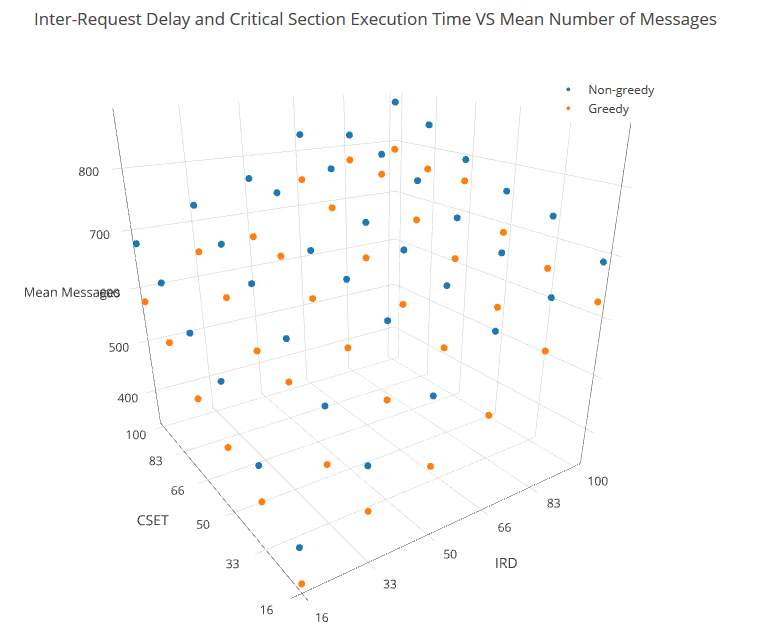
\includegraphics[width=\textwidth]{figs/IRDCSETvsMNM} \\
\end{center}

The above plot shows the relationship between the two input parameters, inter-request delay (IRD, in milliseconds) and critical section execution time (CSET, in milliseconds), and the number of messages sent throughout the network. These tests were run on a perfect 31-node binary tree, with the token starting at the root of the tree. Each data point represents the average of three separate runs with the same configuration. Greedy and non-greedy runs are plotted in orange and blue, respectively. In general, the greedy version outperforms the non-greedy version on this metric, with both seeing a linear increase in the number of messages sent as either IRD or CSET are increased. For an interactive version of this plot, \href{https://plot.ly/~tgduckworth/3/#plot}{visit this webpage.}

\begin{center}
    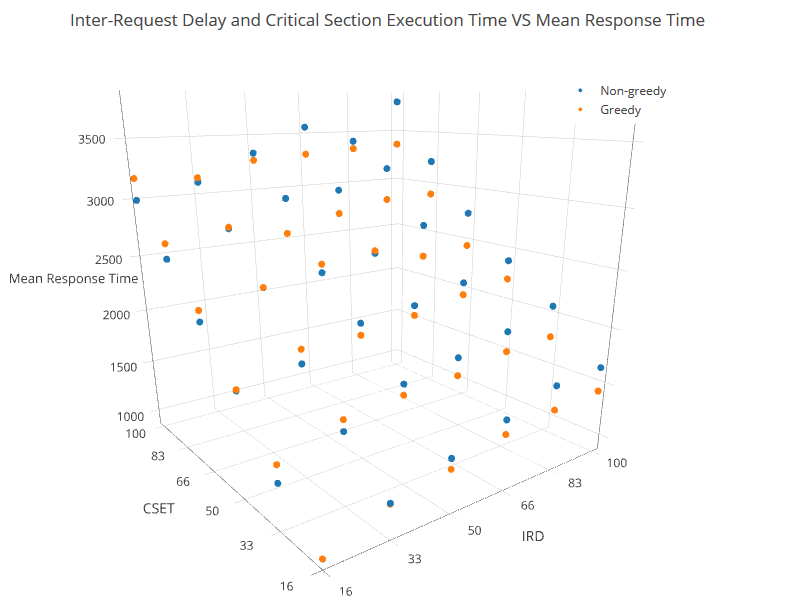
\includegraphics[width=\textwidth]{figs/IRDCSETvsMRT} \\
\end{center}

The above plot shows the relationship between IRD, CSET, and the response time in milliseconds experienced by applications using the system. These tests were run on a perfect 31-node binary tree, with the token starting at the root of the tree. Each data point represents the average of three separate runs with the same configuration. Greedy and non-greedy runs are plotted in orange and blue, respectively. For IRD values above 50, the greedy version tends to be superior, with the non-greedy version performing better for low IRD values. The CSET value dominates the relationship with the response time in a linear relationship, while increasing IRD values only slightly impact this metric. For an interactive version of this plot, \href{https://plot.ly/~tgduckworth/5/}{visit this webpage.}

\begin{center}
    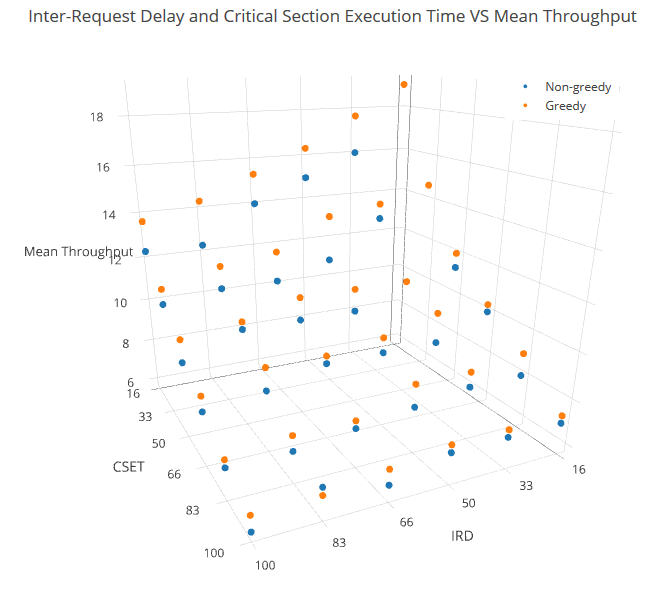
\includegraphics[width=\textwidth]{figs/IRDCSETvsMT} \\
\end{center}

The above plot shows the relationship between IRD, CSET, and the network throughput in requests satisfied per second. These tests were run on a perfect 31-node binary tree, with the token starting at the root of the tree. Each data point represents the average of three separate runs with the same configuration. The greedy version dominates the non-greedy version on this performance measure. Note that the axes, from this perspective, decrease as they move away from us. As CSET decreases, network throughput increases linearly. Decreasing the IRD has a similar effect. For an interactive version of this plot, \href{https://plot.ly/~tgduckworth/6/}{visit this webpage.}

\section{Plotting Diameter/Number of Nodes Against Metrics}

All graphs are plotted with the following fixed parameters:

\begin{itemize}
    \item Inter Request Delay: 20ms
    \item CS Execution time: 5ms
    \item The topology follows a set of perfect binary trees with increasing number of nodes (config files attached: config\_binary3, config\_binary7, config\_binary15, config\_binary31)
    \item Each point in the graph represents an average of 5 runs for each greedy and non-greedy algorithm.
    \item The Red line indicates greedy algorithm execution.
    \item The Blue line indicates Non-Greedy algorithm execution.
    \item (Other results attached with CSV files: Results for Graph.csv, Results of execution.csv)
\end{itemize}

Plot 1 represents a comparison of greedy and non-greedy algorithms for the two parameters: Diameter and the Total number of messages. \\

\begin{center}
    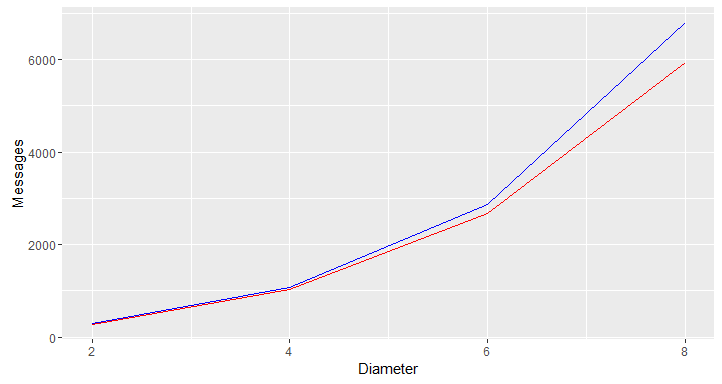
\includegraphics[width=\textwidth]{figs/Plot1} \\
\end{center}

Plot 2 represents a comparison of greedy and non-greedy algorithms for the two parameters: Diameter and the Average number of messages per node. \\

\begin{center}
    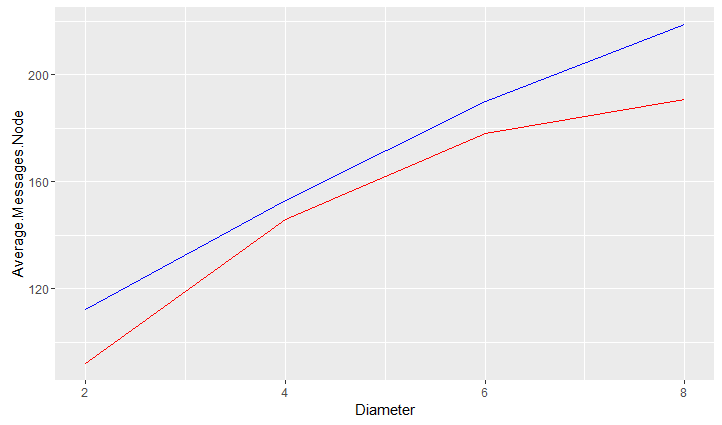
\includegraphics[width=\textwidth]{figs/Plot2} \\
\end{center}

Plot 3 represents a comparison of greedy and non-greedy algorithms for the two parameters: Total Number of nodes and the Total number of messages. \\

\begin{center}
    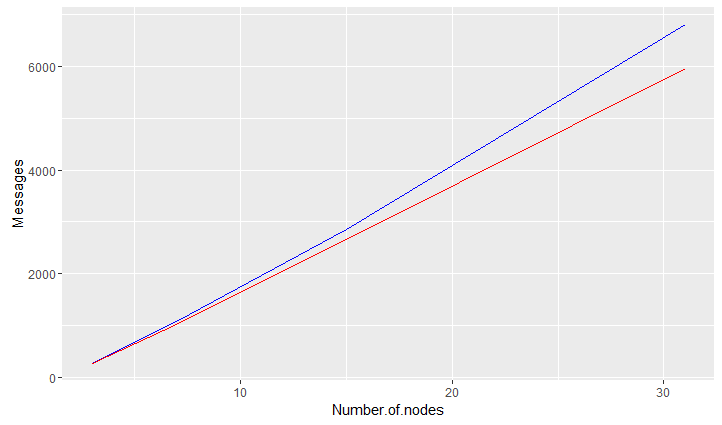
\includegraphics[width=\textwidth]{figs/Plot3} \\
\end{center}

Plot 4 represents a comparison of greedy and non-greedy algorithms for the two parameters: Total number of nodes and the Average number of messages per node. \\

\begin{center}
    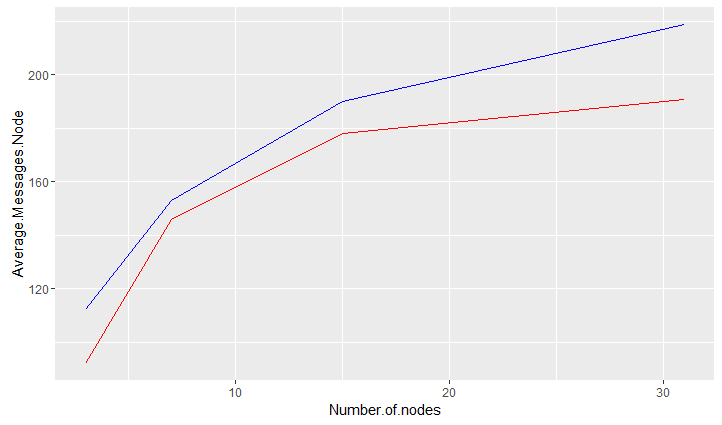
\includegraphics[width=\textwidth]{figs/Plot4} \\
\end{center}

Plot 5 represents a comparison of greedy and non-greedy algorithms for the two parameters: Total number of nodes and the Average throughput of the system. \\

\begin{center}
    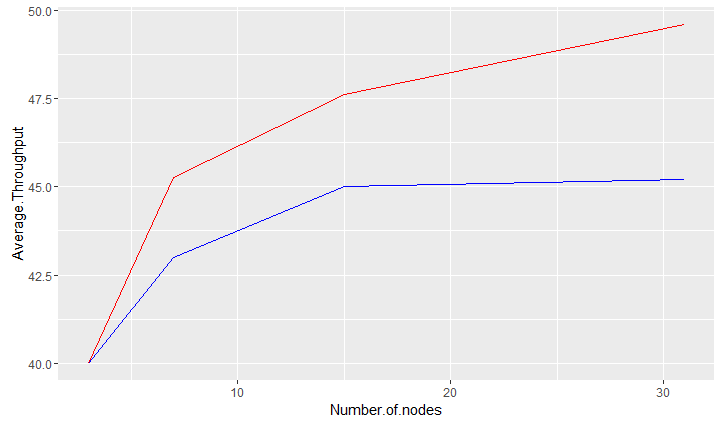
\includegraphics[width=\textwidth]{figs/Plot5} \\
\end{center}

Plot 6 represents a comparison of greedy and non-greedy algorithms for the two parameters: Total number of nodes and the Average Response time. \\

\begin{center}
    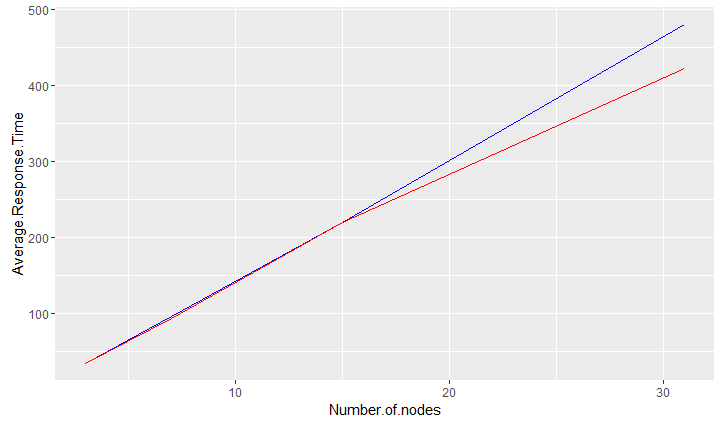
\includegraphics[width=\textwidth]{figs/Plot6} \\
\end{center}

\end{document}